\documentclass[12pt]{article} \setlength{\oddsidemargin}{0in}
\setlength{\evensidemargin}{0in} \setlength{\textwidth}{6.5in}
\setlength{\parindent}{0in} \setlength{\textwidth}{16cm}
\setlength{\topmargin}{1in} \addtolength{\topmargin}{-1.5in}
\setlength{\textheight}{23cm} \setlength{\parskip}{0.75cm}

% Brackets
\usepackage{mathtools} \DeclarePairedDelimiter\ceil{\lceil}{\rceil}
\DeclarePairedDelimiter\floor{\lfloor}{\rfloor}

% Tikz settings
\usepackage{tikz} \usetikzlibrary{trees} \usetikzlibrary {positioning}
\definecolor {mypurple}{cmyk}{0.6,0.4,0.1,0} \definecolor
{myred}{cmyk}{0,0.3,0.3,0} \usetikzlibrary{fit,shapes.misc}

% Typesetting options
\usepackage{fancyvrb} \usepackage{amsmath,amsfonts,amssymb}
\usepackage [english]{babel} \usepackage{url} \usepackage{qtree}

\usepackage{graphicx}
\graphicspath{ {images/} }

\begin{document}

\noindent CSCI 3104 Spring 2018 \hfill Problem Set 5\\
Cole Schlisner (02/22)

\hrulefill

{\fontfamily{cmr}\selectfont

  % ******************* PROBLEM 1 *********************
  \section*{Problem 1}

  \textit{(15 pts) Bellatrix Lestrange is writing a secret message to Voldemort and wants to
prevent it from being understood by meddlesome young wizards and Muggles. She
decides to use Huffman encoding to encode the message. Magically, the symbol frequencies of the message are given by the Pell numbers, a famous sequence of integers
known since antiquity and related to the Fibonacci numbers. The \textbf{n}th Pell number is
defined as $P_n = 2 P_{n-1} + P_{n-2}$ for $n > 1$ with base cases $P_0 = 0$ and $P_1 = 1$.}

  \begin{enumerate}
  \item[(a)]{\textit{For an alphabet of $ \Sigma = \{a, b, c, d, e, f, g, h\}$ with frequencies given by the first $|\Sigma|$ non-zero Pell numbers, give an optimal Huffman code and the corresponding
encoding tree for Bellatrix to use.}}
    \\\\
    $|\Sigma| = 8$\\\\
    $\{P_n | n \in [1 .. 8]\} = [1,2,3,12,29,70,169,408]$\\\\
    $\implies f_a = 1, f_b = 2, f_c = 12, ..., f_h = 408$\\\\
    \textbf{Encodings:}\\
    a: 0000000 \\
    b: 0000001 \\
    c: 000001 \\
    d: 00001 \\
    e: 0001 \\
    f: 001 \\
    g: 01 \\
    h: 1 \\
    \newpage 
    \textbf{Encoding Tree (frequencies of symbols are in parentheses):}\\
    \Tree[.696  [.h(408) \textit{1} ]
                [.288 [.g(169) \textit{01} ]
                      [.119 [.f(70) \textit{001} ]
                            [.49 [.e(29) \textit{0001} ]
                                  [.20 [.d(12) \textit{00001} ]
                                        [.8 [.c(5) \textit{000001} ]
                                            [.3 [.b(2) \textit{0000001} ]
                                                [.a(1) \textit{0000000} ]]]]]]]] \\\\
    Because $P_n > P_{n-1}$, the last symbol in $\Sigma$ should always have the shortest encoding since it always has the highest frequency. The second to last should have the second shortest encoding, etc.
    \newpage
  \item[(b)]{\textit{Generalize your answer to (1a) and give the structure of an optimal code when
the frequencies are the first n non-zero Pell numbers.}}
    \\\\
    The optimal code for this frequency pattern will always resemble what is essentially a linked list as in (1a). This comes from the fact that $P_n > P_{n-1} + P_{n-2}$ by definition. In other words, the meta-symbol created by combining the two symbols with lowest frequencies will always be the lowest frequency symbol in the heap - so there cannot be two branches of the tree with equal frequencies. \\\\
    Except for the first symbol, encoding of symbol at index $i$ (starting at i=1) in $\Sigma$ with $n$ elements whose frequencies are given by the Pell sequence is: 
        \[ \begin{cases} 
          (n-i)\text{x}0 + 1 & i > 1 \\
          (n-i)\text{x}0 & i = 1 
        \end{cases}
    \] [$(n-1)$x$0+1$ = ($n-1$) 0's followed by a 1] \\
  \end{enumerate}

  \newpage

  % ******************* PROBLEM 2 *********************
  \section*{Problem 2}

  \textit{(30 pts) A good hash function $h(x)$ behaves in practice very close to the uniform hashing
assumption analyzed in class, but is a deterministic function. That is, $h(x) = k$ each
time $x$ is used as an argument to $h(x)$. Designing good hash functions is hard, and a
bad hash function can cause a hash table to quickly exit the sparse loading regime by
overloading some buckets and under loading others. Good hash functions often rely
on beautiful and complicated insights from number theory, and have deep connections
to pseudorandom number generators and cryptographic functions. In practice, most
hash functions are moderate to poor approximations of uniform hashing.}

\textit{Consider the following hash function. Let $U$ be the universe of strings composed of the
characters from the alphabet $\Sigma = [A, \dots ,Z]$, and let the function $f(x_i)$ return the index
of a letter $x_i \in \Sigma$, e.g., $f(A)=1$ and $f(Z)=26$. Finally, for an \textbf{m}-character string
$x \in \Sigma^m$, define $h(x)=([\sum_{i=1}^m f(x_i)] \ \text{mod} \ l)$, where $l$ is the number of buckets in the hash table. That is, our hash function sums up the index values of the characters of a
string $x$ and maps that value onto one of the $l$ buckets.}
\newpage
\begin{enumerate}
\item[(a)]{\textit{The following list contains US Census derived last names:}
    
    \textit{\texttt{http://www2.census.gov/topics/genealogy/1990surnames/dist.all.last}}

    \textit{Using these names as input strings, first choose a uniformly random 50\% of these
      name strings and then hash them using $h(x)$.}

    \textit{Produce a histogram showing the corresponding distribution of hash locations
      when $l = 200$. Label the axes of your figure. Briefly describe what the figure
      shows about $h(x)$, and justify your results in terms of the behavior of $h(x)$. Do
      not forget to append your code.}

    \footnotesize{\textit{Hint: the raw file includes information other than name strings, which will need to be removed; and, think about how you can count hash locations without building or using a real hash table.}}
  }
  \\\\
  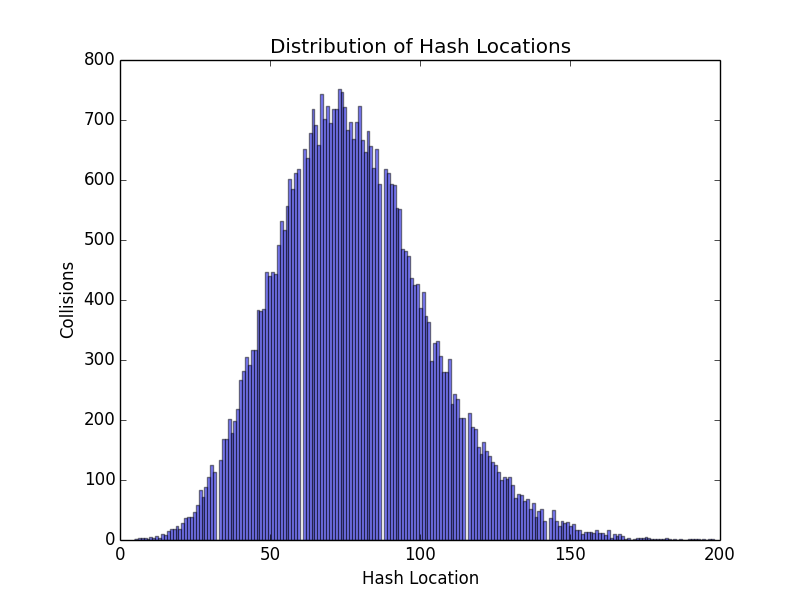
\includegraphics[width=15cm,height=10cm]{figure_1}
  The above histogram illustrates how many collisions occur at each location in the hash table for a random sample of last names. Clearly, it is a bell curve which means given a random name, it is more likely to be hashed into the locations from 50-100 than anywhere else in the table. This means our hashing function h(x) performs pretty poorly, because every location in the table does not have a near equal chance of being mapped to. The ideal h(x) would produce a histogram in which each bar is of equal height, and the bars are equally spread out across hashing locations. 

\pagebreak 

\item[(b)]{\textit{Enumerate at least 4 reasons why $h(x)$ is a bad hash function relative to the ideal behavior of uniform hashing.}}
  \\\\
  \begin{itemize}
    \item[(1)] Not every location has an equal chance of being hashed to, because we have assigned fixed values that scale linearly to each possible input (i.e. the average of 1-26 is 13.5, so we can expect multiples of 13.5 to show up more than other values in h(x) on average)
    \item[(2)] Similar looking inputs will map to similar locations
    \item[(3)] As long as the letters are balanced on each side of the alphabet there are plently of ways to get the same character sum with different strings
    \item[(4)] The hash is heavily affected by the type of input (i.e. for english, a lot of the input uses the same letters with the same frequencies)
  \end{itemize}

\pagebreak
  
\item[(c)]{\textit{Produce a plot showing (i) the length of the longest chain (were we to use chaining for resolving collisions) as a function of the number $n$ of these strings that we hash
into a table with $l = 200$ buckets, and (ii) the exact upper bound on the depth
of a red-black tree with $n$ items stored.}

\textit{Then, (i) comment on the value of $n$ at which the red-black tree becomes a more
efficient data structure, and (ii) state the length of the longest chain when every
bucket has at least one hash hit.}}
  \\\\
  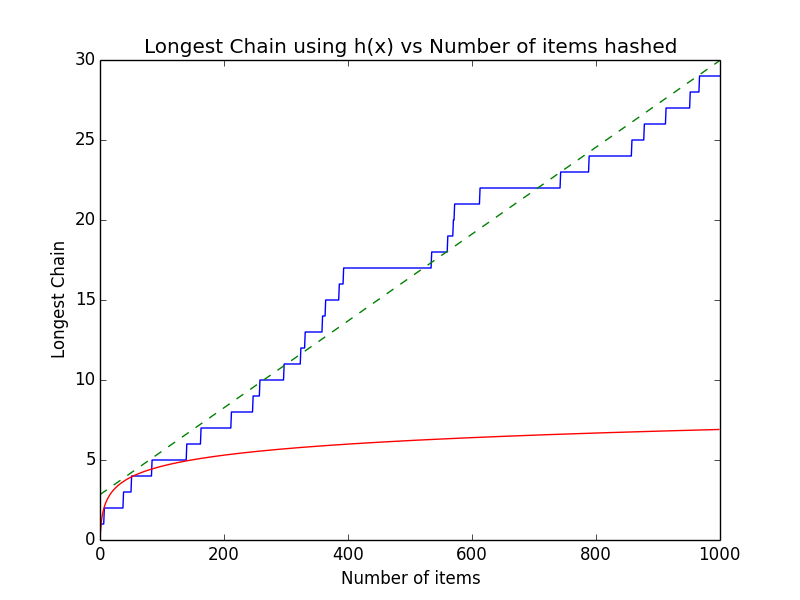
\includegraphics[width=15cm,height=10cm]{figure_2}

  The blue line is the longest chain length, the green line is a best-fit linear function for the longest chain line, and the red line is log(n) - the upper bound for the depth of a red-black tree with n nodes.\\\\
  The red black tree becomes a more efficient data structure at around 83 items - where the blue line crosses the red. \\\\
  If h(x) resembled a good hash function, the amount of items needed to fill all 200 buckets would be approximately $l\text{log}(l) = 200\text{log}(200) \approx 1060$. However when filled with ~44000 items, there still remained 15 or so unfilled buckets. After experimentation, the number of items needed to fill every bucket with the given hash function (using randomly generated strings of length $\le 10$) was around 6.5 million. The longest chain at this point was around 100000. 

\end{enumerate}

\newpage

% ******************* PROBLEM 3 *********************
\section*{Problem 3}

\textit{Draco Malfoy is struggling with the problem of making change for $n$ cents
using the smallest number of coins. Malfoy has coin values of $v_1 < v_2 < \dots < v_r $ for r
coins types, where each coin's value $v_i$ is a positive integer. His goal is to obtain a set
of counts $\{ d_i \}$, one for each coin type, such that $\sum_{i=1}^r d_i=k$ and where $k$ is minimized.}

\begin{enumerate}
\item[(a)]{\textit{A greedy algorithm for making change is the \textbf{cashier's algorithm}, which all young wizards learn. Malfoy writes the following pseudocode on the whiteboard
to illustrate it, where $n$ is the amount of money to make change for and v is a
vector of the coin denominations:}
}

\begin{verbatim}
wizardChange(n,v,r) :
  d[1 .. r] = 0
  // initial histogram of coin types in solution
  while n > 0 {
    k = 1
    while ( k < r and v[k] > n ) { k++ }
    if k==r { return 'no solution' }
    else { n = n - v[k] }
  }
  return d
\end{verbatim}

\textit{Hermione snorts and says Malfoy's code has bugs. Identify the bugs and explain
why each would cause the algorithm to fail.}
    \begin{itemize}
      \item The algoritm iterates from $k=1$ to $r$, meaning it uses the lowest value coins first. This leads to non-optimal solutions every time. Fix this by switching the indicies. 
      \item The algorithm will iterate through all denomiations even if there is a better solution by using the same denomination twice in a row. Fix this by moving the decrement/increment logic outside of the indexing loop.
      \item d is never updated, so the returned array will always be [0 ... 0]. Increment d[k] when n is decremented.
      \item k is incremented before v[k] is used, so the first coin denomination is never used to make change. Move the incrementation/decrementation to the bottom of the loop.
      \item The condition $k<r$ implies the last coin will never be used, make it $k<=r$ (or rather $k >= 1$ with the switched index)
      \item The condition: $k==r$ will never be met, as the enclosing while loop has a condition: $k<r$. Thus "no solution" is unreachable. The only way to know if there is no solution is if n < 0. 
  \end{itemize}

\pagebreak

Correct pseudocode for the greedy algorithm is:\\
\begin{verbatim}
wizardChange(n,v,r){
  d[1..r] = 0
  while n > 0 { 
    k = r
    while ( k >= 1 and v[k] > n){ 
      k -= 1
    }
    n = n - v[k]
    d[k] += 1
  }
  if (n < 0) return 'no solution'
  return d
}
\end{verbatim}

\pagebreak

\item[(b)]{\textit{Sometimes the goblins at Gringotts Wizarding Bank run out of coins\footnote{It's a little known secret, but goblins like to eat the coins. It isn't pretty for the coins, in the end.} and make change using whatever is left on hand. Identify a set of U.S. coin denominations
for which the greedy algorithm does not yield an optimal solution. Justify your
answer in terms of optimal substructure and the greedy-choice property. (The set
should include a penny so that there is a solution for every value of $n$.)}}
  \\\\
  I don't know.
  \\
\item[(c)]{\textit{(8 pts extra credit) On the advice of computer scientists, Gringotts has announced that they will be changing all wizard coin denominations into a new set of coins
denominated in powers of $c$, i.e., denominations of $c^0$, $c^1$, $\dots$, $c^l$ for some integers
$c > 1$ and $l \ge 1$. (This will be done by a spell that will magically transmute old
coins into new coins, before your very eyes.) Prove that the cashier's algorithm
will always yield an optimal solution in this case.}

\footnotesize{\textit{Hint: first consider the special case of $c = 2$.}}}

\end{enumerate}
% ---------------------------------------------------

\newpage

\textbf{References} \\
\hrulefill
\begin{enumerate}
  \item CLRS
  \item \url{https://pythonspot.com/matplotlib-histogram/}
\end{enumerate}

\newpage

\textbf{Appendix 1} \\
\hrulefill
Python 2.7 code for (2a): \\
\begin{verbatim}
import numpy as np
import matplotlib.mlab as mlab
import matplotlib.pyplot as plt
import string

# original list was downloaded as 'data.txt'
# 'lastnames.txt' was generated with the following unix command: 
# $ cut -d ' ' -f 1 data.txt > lastnames.txt

l = 200 # number of buckets
x = []  # list of locations hashed to

# hashing function h(x)
def h(s):
  charsum = 0
  for c in s:
    charsum += string.ascii_uppercase.index(c) + 1
  return charsum % l

# pick n/2 unique random indexes from [0..n]
totalNames = 88800 
chosenOnes = []
while (len(chosenOnes) < (totalNames/2)):
  randInd = np.random.random_integers(totalNames)
  if randInd not in chosenOnes:
    chosenOnes.append(randInd)

with open("lastnames.txt", 'r') as f: # read names from lastnames.txt
  i=0
  for lname in f:
    i += 1
    if (i in chosenOnes): # filter randomly choosen names by index
      x.append(h(lname.strip())) # add this hash location to the list

n, bins, patches = plt.hist(x, l, normed=0, facecolor='blue', alpha=0.5)
plt.xlabel('Hash Location')
plt.ylabel('Collisions')
plt.title(r'Distribution of Hash Locations')
plt.subplots_adjust(left=0.15)
plt.show()
\end{verbatim}

\newpage

\textbf{Appendix 2} \\
\hrulefill
Python 2.7 code for (2c): \\
\begin{verbatim}
import numpy as np
import matplotlib.mlab as mlab
import matplotlib.pyplot as plt
import string
import math
 
# original list was downloaded as 'data.txt'
# 'lastnames.txt' was generated with the unix command: cut -d ' ' -f 1 data.txt > lastnames.txt

l = 200 # number of buckets
x = []  # list of locations hashed to

xx = [0 for i in range(200)] # number of collisions at each location

longestChain = [0 for i in range(1000)]

# hashing function h(x)
def h(s):
  charsum = 0
  for c in s:
    charsum += string.ascii_uppercase.index(c) + 1
  return charsum % l

# pick n/2 unique random indexes from [0..n]
print("picking random names....")
totalNames = 88800 
chosenOnes = []
while (len(chosenOnes) < 1000):
  randInd = np.random.random_integers(totalNames)
  if randInd not in chosenOnes:
    chosenOnes.append(randInd)

print("hashing....")
with open("lastnames.txt", 'r') as f: # read names from lastnames.txt
  i=0
  for lname in f:
    i += 1
    loc = h(lname.strip())
    xx[loc] += 1 # add this hash location to the list
    if xx[loc] > longestChain[i-1]:
      longestChain[i] = xx[loc]
    else: 
      longestChain[i] = longestChain[i-1]
    if i == len(longestChain)-1:
      break

plt.plot(longestChain)
plt.plot(np.unique(range(len(longestChain))), np.poly1d(np.polyfit(range(len(longestChain)), longestChain, 1))(np.unique(range(len(longestChain)))), "--")
plt.plot([math.log(n) for n in range(1, len(longestChain))])
plt.title(r'Longest Chain using h(x) vs Number of items hashed')
plt.ylabel('Longest Chain')
plt.xlabel('Number of items')
plt.show()
\end{verbatim}

\end{document}